%%This is a very basic article template.
%%There is just one section and two subsections.
\documentclass[twocolumn]{article}
\usepackage{graphicx}
\usepackage{amsmath}
\usepackage{amssymb}
\usepackage{subfigure}
\title{Tuning plasmon of gold nanorods by KCN etching}
\author{Aquiles Carattino \and Pedro Navarro \and Saumya Khatua \and Michel
Orrit}

\begin{document}
\maketitle
\abstract{This is the abstract}

\section{Introduction}
Gold Nanorods (AuNR) are employed in a variety of fields, ranging from solar
cells production\cite{Catchpole:08} to biosensing. These nanoparticles exhibit a
Surface Plasmon Resonance (SPR), i.e., a collective oscillation of the
conduction electrons, that is related to their aspect ratio (AR); spherical
particles (AR=$1$) have the plasmon peak at around $540nm$ while rods can be
tuned to have it even above $900nm$. This tuning is usally done at the time of
the synthesis by varying the concentration of seed and grow solutions. However,
even in the best case, every sample will show a dispersion of both shapes and 
plasmon peak positions.

This work focus in the employment of KCN as an etching agent that will allow to
fine-tune the plasmon peak position. The overall reaction can be written as 

\begin{equation}
4\textrm{Au} + 8\textrm{KCN}^-+\textrm{O}_2 + 2\textrm{H}_2\textrm{O}
\leftrightarrows 4\textrm{Au(CN)}_2^-+4\textrm{KOH}^-
\end{equation}

In bulk this compound is used for reducing the aspect ratio of the rods, i.e.
blue shifting their plasmon. In a more recent paper it was also used for
generating highly spherical particles with a narrow size distribution. 

In this work the opposite trend is observed. Single-particle experiments of the
AuNR immersed in KCN show a red-shift of the plasmon meaning an increase in
aspect ratio. This is confirmed by tracking the spectra of individual rods over
time as well as by acquiring SEM images of them. A simple model where etching is
considered as being isotropic and constant, this means that both the radius of
the particle and it's length diminish at the same rate over time, yields a high
agreement with both sets of experiments. 

\section{Experimental method}
Two kind of experiments are carried on; the first will be called the optical
experiment and consists of acquiring the luminescence spectra of single gold
nanorods (AuNR) in a home built confocal microscope using an Acton 500i
Spectrometer. For exciting the particles a $532nm$ laser is used with a power
in the back focal plane of $300\mu W$. A high NA objective (Olympus $60X NA 1.4$
Oil immersion) is used for both focusing the laser and collecting the
luminescence. A $532nm$ notch filter is used for cutting out the excitation.

The samples are prepared by spin casting a suspention of AuNR on a clean
coverslip and thoroughsly rinsing them  with water for eliminating the excess of
CTAB. The samples are then placed in a flowcell; the initial spectra are taken
with the rods immersed in Milli-Q water. After this, a solution of KCN is flowed
into the cell with concentrations ranging from $3\mu M$ to $50\mu M$. Then the
spectra of several rods is collected by consecutively focusing in different
particles. This allows to track the spectra of approximately $10$ particles
simultaneusly.

The second kind of experiments were performed in an SEM. The samples
were prepared by letting a droplet of a suspension of AuNR dry on top of a
silicon waffer and then thoroughlsy rinsing them with water for eliminating the
excess of CTAB. The same samples are employed for taking images before and after
immersing the particles in $30\mu M$ KCN. Particular care is taken in having the
rods separated from each other as to reproduce the conditions found in the
optical experiment. After immersing the samples in KCN for a given period of
time, they are rinsed with water to stop the reaction.

\section{Results and discussion}
As stated before two experiments are performed, the first in a
confocal microscope and the second in an SEM. These findings are compared to
numerical simulations using the discrete dipole approximation. The first set of
experiments allows to have a high temporal resolution, at the same time that
following the plasmon peak and shape of several AuNR. The second experiment, on
the other hand, allows to gain insight into the real shape of rods in exchange
of a lower temporal resolution. 

\begin{figure}[htb]
 \centering
 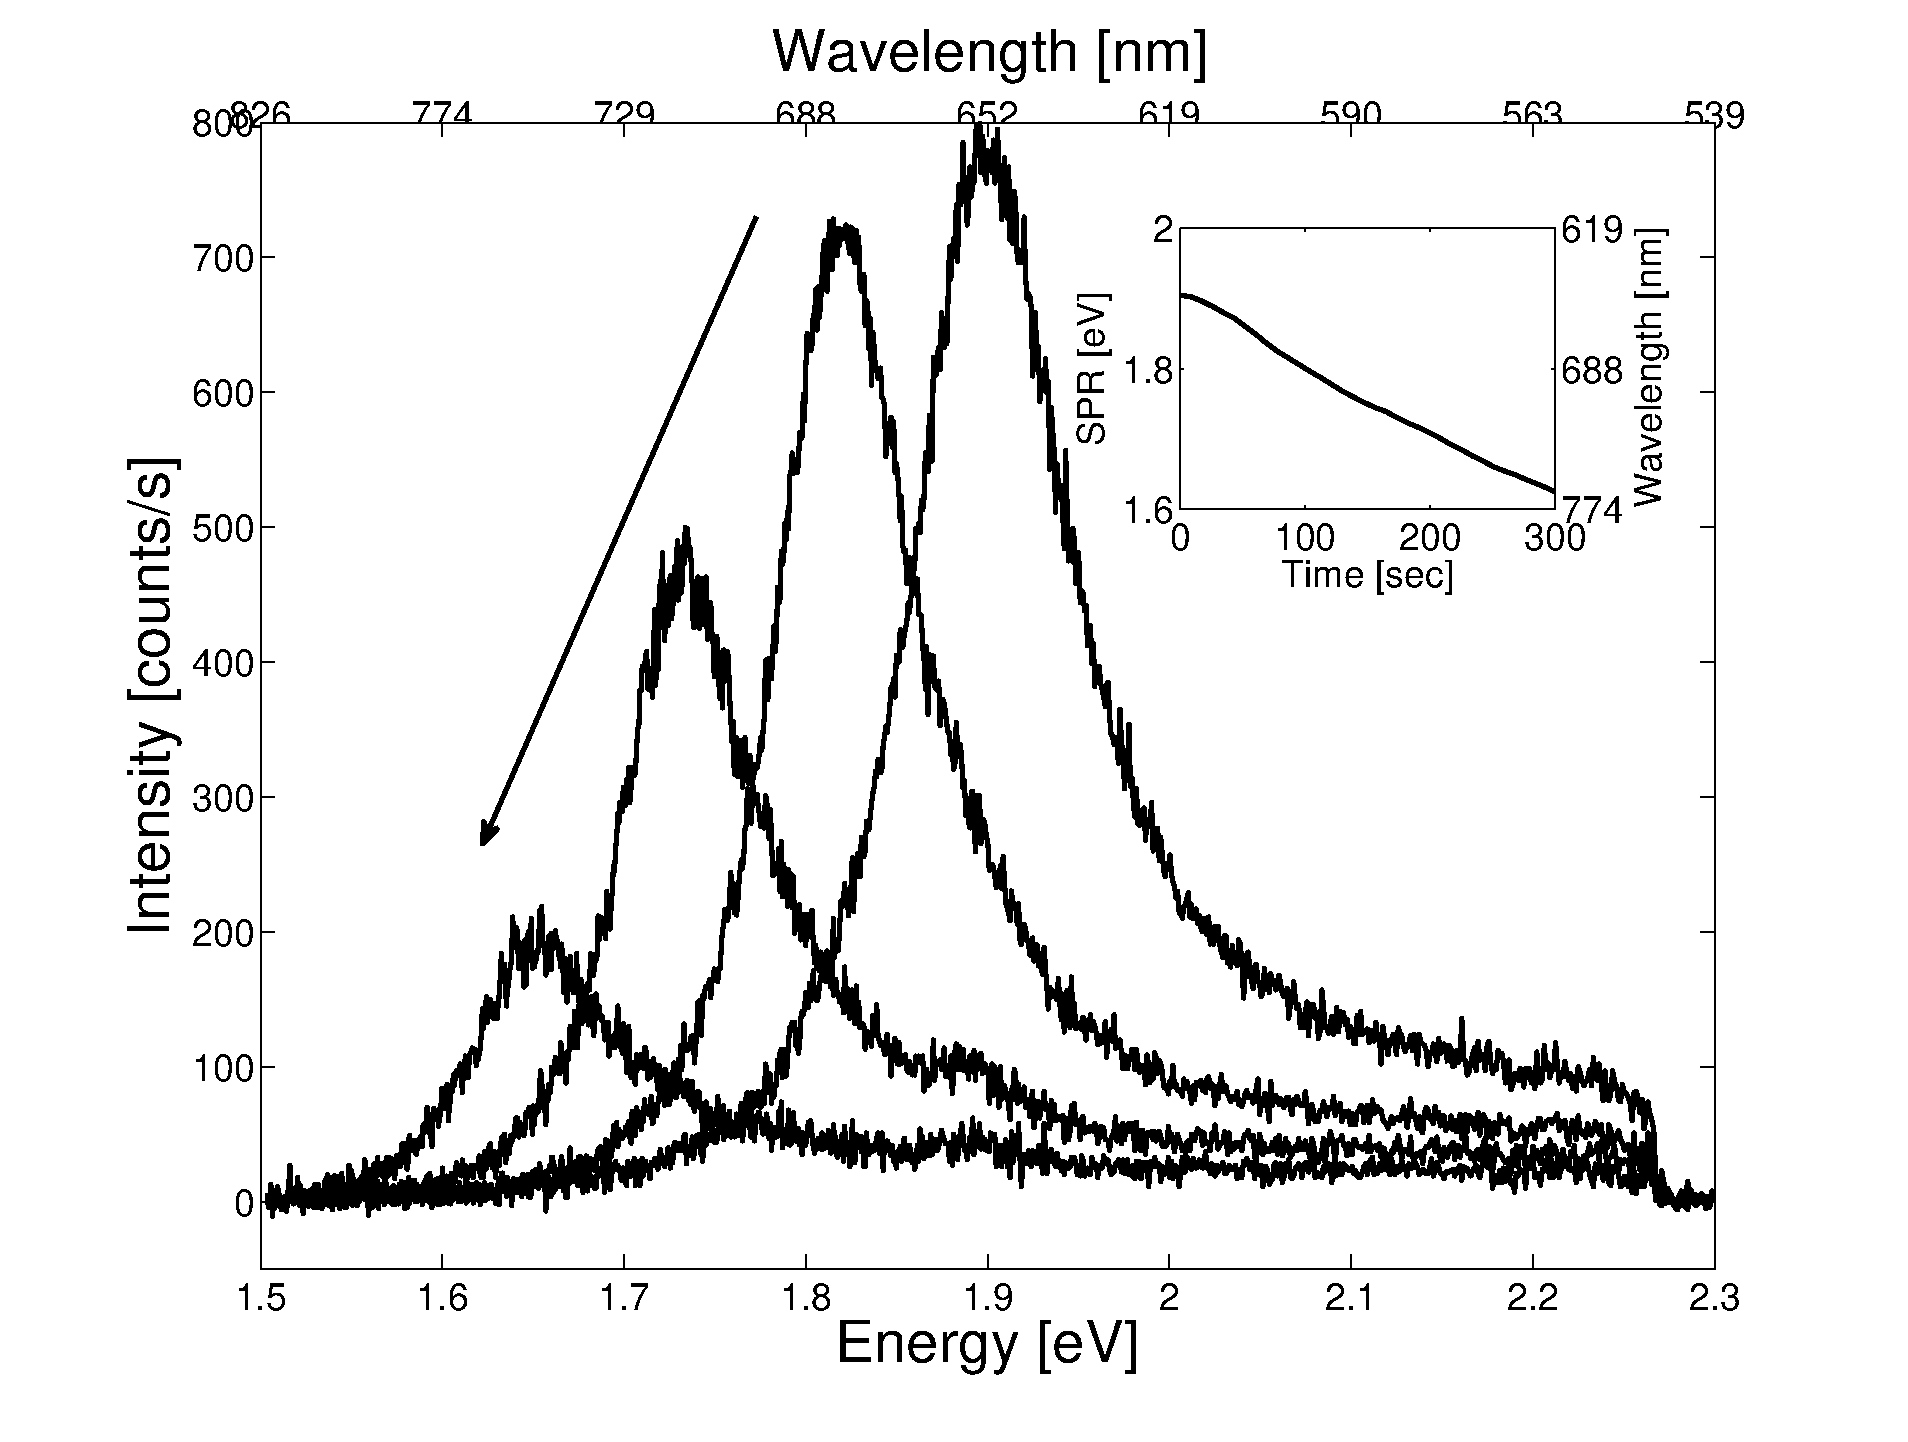
\includegraphics[width=0.9\linewidth]{plasmon_single_rod.eps}
 \caption{Plasmon shift due to the etching with $30\mu M$ KCN. The time
 interval between peaks is $70s$. The inset shows the peak position of the SPR as a
 function of time, extracted by fitting the spectra with a Lorenzian.}
 \label{fig:plasmon_single_rod}
\end{figure}

Figure \ref{fig:plasmon_single_rod} shows the typical behavior of the plasmon of
a single rod while immersed in KCN $30\mu M$. The Figure shows the acquired
spectra with an interval of $70s$ while the inset shows the peak position
(calculated by fitting the spectra with a lorentzian) over time. It can be seen
that the plasmon red-shifts over $100\, nm$ ($0.25\, eV$) in $5$ minutes. The
diminishing intensity is consistent with the volume loss given by the
dissolution of gold. In this case only one rod is observed therefore having a
higher temporal resolution, but exactly the same trend was observed for each
single nanorod.



Figure \ref{fig:SEM_30muM} shows three SEM images for a sample of the same
nanorods used in the optical experiment before the etching, after $2min$
submersed in KCN and after $4min$. It is possible to observe that the AuNR
preserve the shape while diminishing the volume and increasing the aspect ratio.
This enables to perform statistics on the findings, as will be explain
hereafter. 


\begin{figure}[htb]
 \centering
 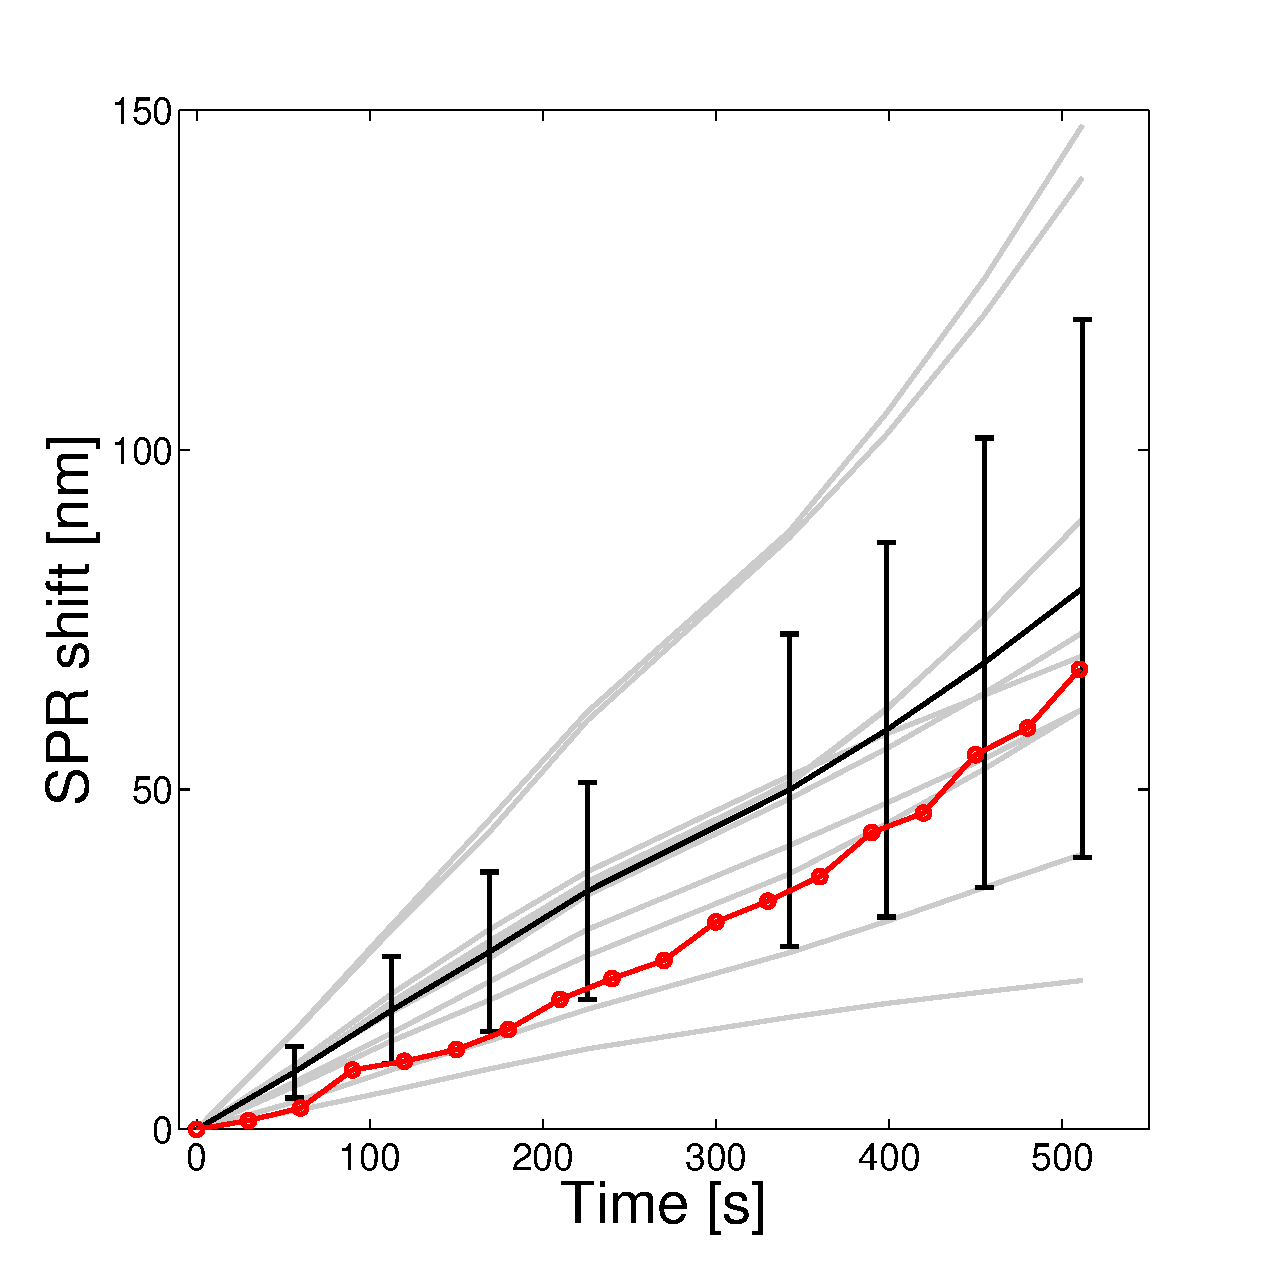
\includegraphics[width=0.9\linewidth]{plasmon_average.eps}
 \caption{Average plasmon shift for 9 rods due to the etching with $30\mu M$
 KCN. The light curves are individual timetraces while the thick one is the
 average. The error bars are simply the standard deviation at each point. Over
 time the peak distribution gets broader.}
 \label{fig:plasmon_average}
\end{figure}

Figure \ref{fig:plasmon_average} shows the timetraces of the peak positions of
$9$ different rods while being etched with $30\mu M$ KCN. The pale lines show
each individual trace, while the darker is the average. The error bars are simply the
standard deviation of the distribution at each point. The bigger time step
between $225s$ and $340s$ is due to an automatic refocusing happening on the
particles every $5\textrm{min}$. 

The red-shift is observed for every particle, at different KCN concentrations.
The broadening of the distribution is also observed and has to be attributed to
intrinsic inhomogenities in the particles since it is not possible to relate it 
nor to the initial particle volume nor to its initial plasmon peak position. 

Figure \ref{fig:plasmon_distribution_sem} shows the aspect ratio distribution of
the AuNR at the beginning, after $2min$ and after $4min$ in KCN. It is possible
to observe that the aspect ratio increases with time and that it's distribution
is getting broader. This is in a direct agreement with what was found in the
optical experiment (i.e. a larger aspect ratio leads to a plasmon position
towards the red and a broadening of the distribution means a broadening in the
plasmon peak position). 

To interpret these results it is possible to calculate the plasmon peak position
together with the size of the particle by using the ADDA package. By checking
the radius and length distribution of the rods in the SEM at different instants, 
it can be assumed an isotropic etching, i.e. both radius and length diminish at
the same rate. Figure \ref{fig:adda_plasmon_shift} shows the shift of the
plasmon peak. The horizontal axis scale was set to match the results of the SEM
(namely, an etching rate of $0.5nm/min$ for a KCN concentration of $30\mu M$).
It is possible to observe a great overlap with what was observed for a single
particle in the optical experiment. 

\section{Conclusions}
In this work it is shown a simple method that allows the tuning of the plasmon
peak position of a gold nanorod with nanometer accuracy. More importantly, it is
shown that the rodlike shape is preserved even for plasmon shifts of
approximately $80nm$ therefore keeping the well known properties of them. 

The optical experiments show the red-shift of the plasmon with a high time
accuracy, while with the SEM it is possible to confirm that the shape of the
rods is being preserved. The agreement between the simulations and the
experimental results not only show the link between both measurments but also
provide a way of predicting the behaviour of the plasmon peak. 

Tuning the resonance of plasmonic structures after the synthesis of the
particles and moreover after fixing them on a substrate are of great interest
for a diversity of experiments where, for instance, there is the need of
overlapping the particle spectra with a fluorophore or with the wavelenght of
the available lasers.

\bibliography{bibliography}{}
\bibliographystyle{plain}

\end{document}
